% !TeX encoding = UTF-8
% IEEE conference draft: original English/Chinese content; no figures.
\RequirePackage{iftex}
% Preserve the original class's pdfLaTeX layout calculation before changing
% only the text encoding needed for the bilingual draft.
\ifPDFTeX\else
  \RequirePackage[T1]{fontenc}
\fi
\documentclass[conference]{IEEEtran}
\ifPDFTeX
  \usepackage[T1]{fontenc}
\fi
\usepackage{cite}
\usepackage{amsmath,amssymb,amsfonts}
\usepackage{textcomp}
\usepackage{booktabs}
\usepackage{tabularx}
\usepackage{array}

% Keep the default pdfLaTeX workflow working. Select Chinese support
% according to the active engine instead of unconditionally loading xeCJK.
\ifPDFTeX
  \usepackage{CJKutf8}
  \newcommand{\StartChinese}{\begin{CJK*}{UTF8}{gbsn}}
  \newcommand{\StopChinese}{\clearpage\end{CJK*}}
\else
  % ctex selects xeCJK for XeLaTeX and luatexja for LuaLaTeX.
  % scheme=plain preserves the IEEE heading and layout definitions.
  \usepackage[UTF8,scheme=plain,fontset=fandol]{ctex}
  \setmainfont{texgyretermes}[Extension=.otf,UprightFont=*-regular,BoldFont=*-bold,ItalicFont=*-italic,BoldItalicFont=*-bolditalic]
  \setsansfont{texgyreheros}[Extension=.otf,UprightFont=*-regular,BoldFont=*-bold,ItalicFont=*-italic,BoldItalicFont=*-bolditalic]
  \setmonofont{texgyrecursor}[Extension=.otf,UprightFont=*-regular,BoldFont=*-bold,ItalicFont=*-italic,BoldItalicFont=*-bolditalic]
  \newcommand{\StartChinese}{}
  \newcommand{\StopChinese}{}
\fi

\begin{document}
\StartChinese
\title{VLA inference with LPDDR PIM}
\author{}
\maketitle

\begin{abstract}
% Source: # Abstract
% Template-neutral migration fragment; original wording retained.
Vision-Language-Action (VLA) models are central to embodied AI, but strict real-time inference on resource-constrained edge platforms remains challenging. A typical VLA model cascades a relatively compute-intensive Vision-Language Model (VLM) and a memory-bound Action Expert (AE). While VLM and AE support asynchronous parallelism algorithmically, running them concurrently via dual streams on a single GPU yields negligible speedup, motivating heterogeneous hardware. 

In this work, we propose VLA-PIM, a heterogeneous GPU-LPDDR5X-PIM architecture–dataflow co-design for edge VLA inference. VLA-PIM uses rank-level partitioning to co-execute the VLM on the GPU and the AE on LPDDR-PIM. However, shared-bus contention limits GPU–PIM concurrency, as conventional PIM execution leaves fragmented bus idle windows and heavily occupies the bus with frequent inter-rank data transfer. To resolve this, we co-design an input-preloading microarchitecture and a DQ-aware dataflow, increasing the bus cycles available to the GPU by 34\%. Evaluation combining Ramulator-based cycle-accurate simulation and NVIDIA Thor measurements demonstrates a $1.82\times$ latency reduction and $2.55\times$ energy reduction over a GPU baseline. We open-source our code at https://anonymous.4open.science/r/vla-pim-paper-artifact/.
\end{abstract}

% Source: 文章_bu1118.docx, Introduction only.
\section{Introduction}
\label{sec:introduction}

Vision-Language-Action (VLA) models have become a core paradigm for general-purpose embodied AI by mapping multimodal perceptions and language instructions into robot actions. However, practical VLA deployment faces severe challenges. While VLA inference must meet strict real-time constraints to avoid task failure, the physical limits of robots restrict deployment to edge platforms with constrained power, compute, and memory bandwidth, such as the LPDDR-equipped NVIDIA Orin and Thor. Taking the representative $\pi_{0.5}$ model~\cite{pi05} as an example, its inference latency on NVIDIA Thor reaches about $141\,\mathrm{ms}$ ($7\,\mathrm{Hz}$), limiting the robot's control frequency.

From a workload perspective, VLA models show heterogeneity in computation and memory access~\cite{vla_perf}. A typical VLA model cascades a Vision-Language Model (VLM) and an Action Expert (AE), with an execution time ratio of about 1:1 to 1:2 (\textbf{Fig.~\ref{fig:intro-overlap}(a)}). As embodied robot control dictates single-batch inference, the large difference in input token lengths between the two networks leads to distinct operational intensities (OI). Profiling on NVIDIA Thor shows that the AE is severely memory-bound, while the VLM lies near the boundary between the compute- and memory-bound regions (Section~\ref{sec:background-a}). Although recent works decouple sequential VLM--AE execution into asynchronous parallel execution to hide latency~\cite{vla_xpu,ravel}, single-GPU concurrency fails to exploit this algorithmic parallelism because streaming the AE saturates the off-chip memory bandwidth, achieving only a $1.03\times$ speedup via dual-stream execution on NVIDIA Thor (\textbf{Fig.~\ref{fig:intro-overlap}(b)}).

% Source: figures/sources/figures1107-20261118.pdf, page 1.
% PDF content retained; only blank page borders cropped.
\begin{figure}[!tb]
\centering
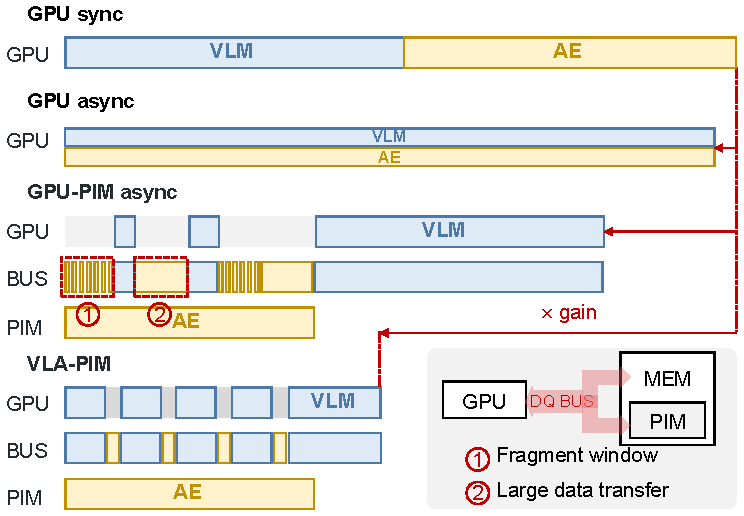
\includegraphics[width=\columnwidth,pagebox=cropbox]{figures/execution-overview.pdf}
\caption{VLA execution paradigms: serial GPU execution, GPU--PIM overlap limited by fragmented bus windows and data transfers, and VLA-PIM.}
\label{fig:intro-overlap}
\end{figure}


Achieving effective VLM--AE parallelism for such heterogeneous workloads requires heterogeneous hardware. DRAM Processing-in-Memory (PIM)~\cite{rowclone,ambit,fimdram,upmem_prism} can efficiently accelerate memory-bound workloads by computing near the memory arrays. Therefore, replacing the edge GPU's standard LPDDR with LPDDR-PIM offers an attractive heterogeneous solution: LPDDR-PIM can supply main-memory data to the GPU for VLM execution while concurrently computing the memory-bound AE in memory to hide latency.

However, because GPU memory accesses and PIM transfers share the same command/address (C/A) and data (DQ) buses of the LPDDR interface, efficient GPU--PIM concurrency is severely limited by shared-bus contention (\textbf{Fig.~\ref{fig:intro-overlap}(c)}). This contention stems from two main aspects. First, PIM's streaming input and execution leave highly fragmented bus idle windows. Overly short windows cannot accommodate complete GPU memory accesses, while fragmented windows force frequent PIM-to-GPU rank switching, incurring high turnaround overhead. Second, massive inter-rank PIM data movement heavily occupies the bus. Specifically, executing the AE on PIM involves matrix transposition, data rearrangement, broadcast, and partial-sum reduction, all of which require frequent inter-rank communication.

Prior GPU--PIM coordination techniques cannot resolve this contention under edge LPDDR constraints. Some designs (e.g., AHASD and LP-Spec~\cite{ahasd,lp_spec}) add cross-rank global schedulers and memory controllers (MCs) that rely on a \emph{logic die}, which is absent in commercial LPDDR and Samsung's LPDDR-PIM~\cite{samsung_lpddr5x_pim}. Other designs that invasively modify internal bank circuits on the DRAM die for concurrent access and computation (e.g., NeuPIMs~\cite{neupims}) incur prohibitive area overhead, over $10\times$ higher than logic-die implementations~\cite{sangam,devaux}.

In this work, we present VLA-PIM (\textbf{Fig.~\ref{fig:intro-overlap}(d)}), the first heterogeneous GPU-LPDDR5X-PIM system that accelerates edge VLA inference through architecture--dataflow co-design. Specifically, VLA-PIM employs rank-level partitioning to isolate memory resources between GPU accesses and PIM computation (Section~\ref{sec:architecture-a}). Furthermore, an input-preloading microarchitecture (Section~\ref{sec:architecture-b}) and a DQ-aware dataflow (Section~\ref{sec:dataflow-a}) mitigate shared-bus contention, effectively overlapping AE computation with VLM execution. Notably, VLA-PIM requires neither a \emph{logic die} nor invasive bank modifications while matching the compute and local-buffer budgets of Samsung's LPDDR-PIM, ensuring practical hardware feasibility. Our contributions are summarized as follows:

\begin{itemize}
\item We characterize the distinct OI of the VLM and AE, and introduce a heterogeneous execution paradigm that runs the VLM on the GPU and the AE on PIM in parallel.
\item We propose the VLA-PIM architecture, which employs rank-level resource partitioning to isolate GPU memory accesses for the VLM from in-memory PIM execution for the AE with minimal hardware overhead.
\item We design an input-preloading microarchitecture to eliminate fragmented bus windows, alongside a DQ-aware dataflow to minimize inter-rank traffic on the shared bus.
\end{itemize}

We build and open-source a Ramulator-based cycle-accurate simulator~\cite{ramulator2} to evaluate VLA-PIM, demonstrating a $1.82\times$ speedup and a $2.52\times$ energy reduction over a serial GPU baseline.

% Source: ## II 背景与动机
% Template-neutral migration fragment; original wording retained.
\section{BACKGROUND AND MOTIVATION}
\label{sec:background}

\subsection{Execution Characteristics and Bandwidth Bottlenecks of Asynchronous VLAs}
\label{sec:background-a}

Embodied Vision-Language-Action (VLA) models, exemplified by $\pi_{0.5}$, typically couple a Vision-Language Model (VLM) with an Action Expert (AE): the VLM encodes multimodal observations (images and language instructions), while the AE reuses this context to generate action chunks via multi-step denoising (Fig.~1(a)). However, AE inference accounts for over half of the total execution latency (Fig.~1(b)), severely bottlenecking the system control frequency. To mitigate this, recent works adopt asynchronous pipelining, allowing the AE to generate actions from a ready context concurrently as the VLM processes incoming observations. In an ideal two-stage pipeline, the per-step latency shrinks from the sum of both stages down to that of the bottleneck stage.

In practice, however, limited off-chip memory bandwidth on edge GPUs severely undermines this pipelining benefit. As shown in the Roofline analysis (Fig.~1(c)), the AE processes few action tokens with minimal weight reuse, resulting in low operational intensity (OI) and strictly memory-bound behavior. Although the VLM processes substantially more visual and text tokens with higher OI—operating closer to the ridge point of target edge platforms such as NVIDIA Thor—most of its operators still fall within the memory-bound regime. Consequently, concurrent execution triggers severe contention for shared off-chip memory bandwidth. Our profiling on Thor (MHA8 configuration) confirms that even with \texttt{torch.compile} optimization, dual-stream concurrency only reduces execution latency from $141.29\text{ ms}$ to $137.07\text{ ms}$, yielding a negligible $1.031\times$ speedup (Table~\ref{tab:performance}).

These execution characteristics motivate a heterogeneous co-design approach. With ultra-high internal bandwidth and moderate compute capability, Processing-in-Memory (PIM) architectures naturally match the low-OI, memory-bound profile of the AE. Conversely, the VLM exhibits higher OI and compute demand, making it better suited for general-purpose GPUs. Therefore, we offload the AE's primary linear operations to PIM, enabling in-situ access to weights and the KV cache directly inside memory banks. By drastically curtailing data transfers across the external memory bus (i.e., DRAM DQ pins), this partitioning strategy eliminates cross-stage bandwidth contention and frees up critical off-chip bandwidth for the GPU-resident VLM.

\subsection{LPDDR-PIM for Edge Inference}
\label{sec:background-b}

LPDDR combines energy efficiency with compact packaging and serves as main memory in edge platforms such as NVIDIA Orin and Thor~\cite{micron_lpddr}. LPDDR-PIM adds computation within DRAM. Samsung's LPDDR5X-PIM, for example, couples a processing unit with each bank to exploit the aggregate internal bandwidth~\cite{samsung_lpddr5x_pim}.

LPDDR is organized into channels, ranks, and banks. Each channel provides independent command/address (C/A) and data (DQ) buses. Ranks within a channel are selected by separate chip-select (CS) signals and have independent storage arrays, but share the channel's external buses. Within each rank, PIM units access data through local bank paths. The shared buses must therefore serve both GPU memory requests and PIM data transfers.

Existing designs introduce additional hardware to support concurrency. NeuPIMs adds dual row buffers within each bank~\cite{neupims}, while LP-Spec introduces a near-data memory controller, independent command paths, and buffers~\cite{lp_spec}. These mechanisms do not directly apply to a configuration that retains conventional row buffers and shared C/A and DQ interfaces, motivating alternative ways to manage shared-bus traffic.


\subsection{Challenges of Sharing the LPDDR Bus}
\label{sec:background-c}

Two aspects of PIM communication limit the bandwidth available to the GPU:

\begin{enumerate}
    \item \textbf{Fragmented access windows.}
    Streaming inputs into limited PIM buffers interleaves external transfers with internal computation, leaving short, scattered DQ idle windows. GPU accesses must satisfy cross-rank and read/write turnaround timing constraints. Short windows may not accommodate a useful transfer, while frequent switching reduces efficiency. Consequently, usable GPU bandwidth depends on both the duration and distribution of these windows.

    \item \textbf{Communication overhead from data mapping.}
    Local broadcasts remain within a rank, whereas inter-rank exchanges routed through the host memory controller occupy DQ. Feature-wise partitioning of attention can require such exchanges to combine partial results. Similarly, Q/K tensors produced in PIM must travel to the GPU and back if rotary position embedding (RoPE) is performed there. These transfers recur across denoising steps, increasing AE latency and reducing bandwidth available to the VLM. Data partitioning and operator placement must therefore account for their external communication costs.
\end{enumerate}

These observations motivate VLA-PIM's design: assign GPU memory accesses and AE computation to separate ranks, then combine input preloading with communication-efficient data mapping to reduce external transfers and create contiguous GPU access windows.

% \subsection{异步 VLA 的执行特征与带宽瓶颈}
% \label{sec:background-a}


% 以 \(\pi_{0.5}\)等具身视觉语言动作（VLA）模型为代表的架构通常由视觉语言模型（VLM）与动作专家（AE）协同构成：VLM 负责编码多模态观测（图像与语言指令），AE 则复用其上下文通过多步去噪生成动作块（图 1(a)）。然而，AE 的推理耗时占总体的一半以上（图 1(b)），严重制约了系统的控制频率。为此，现有研究引入异步流水线执行机制——允许 AE 基于已就绪的上下文并行生成动作，同时由 VLM 处理新观测。在理想的双阶段流水中，单轮执行周期可由两阶段耗时之和缩短至接近瓶颈阶段的水平。

% 然而，边缘端 GPU 有限的片外带宽严重削弱了这种流水线重叠效益。如图 1(c) 所示，AE 处理的动作 Token 数量较少、权重复用率低，其核心算子具有较低的算术强度（Arithmetic Intensity, OI），呈现出典型的存储带宽受限（Memory-bound）特征。尽管 VLM 处理的视觉与文本 Token 规模更大、OI 更高且接近目标平台（如 Thor）的 Roofline 模型拐点，但其多数算子仍处于带宽受限区。因此，双阶段并发执行会导致严重的片外内存带宽竞争。我们在 Thor 平台的 MHA8 配置下的实测表明，经 \texttt{torch.compile} 优化后的双 Stream 并发仅将执行延迟从 141.29 ms 微降至 137.07 ms，加速比仅为 1.031\(\times\)（表 I）。

% 基于上述分析，处理内存（PIM）架构凭借极高的内部带宽和适度的算力，非常契合 AE 这类低 OI、访存主导型的计算负载。相比之下，VLM 的算术强度与计算吞吐需求显著更高，更适合保留在通用 GPU 上运行。因此，本文提出异构协同计算方案：将 AE 的主要线性计算卸载至 PIM，使其在存储端直接完成权重与 KV Cache 的读取，从而大幅削减经由外部总线（如 DRAM 的 DQ 引脚）的数据传输量，为 GPU 上的 VLM 释放宝贵的片外带宽。这种软硬件协同的分工策略不仅精准匹配了双阶段的计算特征，也为根本缓解并发场景下的带宽竞争提供了有效途径。

% \subsection{面向边端的 LPDDR-PIM 协同执行}
% \label{sec:background-b}


% 低功耗双倍数据速率内存（LPDDR）兼顾高能效与紧凑封装，是 NVIDIA Orin、Thor 等边缘平台的主流主存方案 (micron.com)。LPDDR-PIM 在此基础上将计算单元直接集成于 DRAM 内部——例如三星提出的 LPDDR5X-PIM 便将处理单元与各 DRAM Bank 一一对应耦合，从而在主存内部提供了直接利用高聚合内部带宽的计算能力。

% 从存储微架构层级来看，LPDDR 的外部总线接口与内部存储阵列呈现出显著的解耦特性：每个通道（Channel）配备独立的命令/地址总线（C/A）与数据总线（DQ），并可挂载多个由片选信号（CS）独立控制的 Rank；同通道内的各 Rank 拥有独立的存储阵列，但在对外接口上共享该 Channel 的 C/A 与 DQ 总线；而在 Rank 内部，存储空间进一步划分为多个 Bank，PIM 逻辑正是通过 Bank 级本地数据通路直接读取阵列数据进行运算。

% 本文的多 Bank 协同计算模式，\textbf{Rank 级划分}最为契合：它能够直接复用现有的 CS 片选机制与独立存储阵列，将 AE 计算与 VLM 访存分别映射至不同 Rank，从而在 PIM 执行片内计算期间，确保所有 Channel 仍能满载响应 GPU 的常规访存请求。

% 为提升并发度，既有研究多依赖激进的硬件微架构改动——例如 NeuPIMs 在 Bank 内增设双行缓冲（Dual Row-buffer），LP-Spec 则引入近存控制器（NMC）、独立 C/A 通路及额外缓冲，均在阵列外围或接口侧引入了不可忽视的面积与控制开销 。本文坚持低侵入性（Low-overhead）设计原则，不引入额外的 Logic Die，完整保留原有的行缓冲组织以及共享的 C/A、DQ 物理接口，仅对 PIM 的局部数据通路进行轻量级扩展。在这一严格的硬件约束下，系统设计的核心便聚焦于如何精简并重排外部总线通信，使 Rank 级物理隔离真正转化为高效的实际并发。

% \subsection{共享总线下的协同挑战}
% \label{sec:background-c}


% 尽管 Rank 级分工为 GPU 保留了全通道访问的物理潜力，但实际可获得的带宽收益仍受制于 PIM 对共享总线的占用模式，主要面临两方面瓶颈：

% \begin{enumerate}
% \item \textbf{访存窗口碎片化与总线时序开销}：受限于 PIM 有限的输入缓冲区，传统的流式供数模式迫使 PIM 交替执行数据接收与计算，导致 DQ 总线上充斥着零散、短暂的空闲窗口。GPU 在此类碎片化窗口内访存，不仅需承受跨 Rank 切换与读写转向的时序开销，过窄的窗口更难以承载有效突发传输，严重拉低总线利用率，LPDDR5X-PIM 的相关技术分析亦证实了细粒度输入写入的显著开销。因此，亟需将 PIM 的外部传输集中调度，为 GPU 留出连续的访存窗口。
% \item \textbf{数据映射决定了 AE 的外部 DQ 通信开销。} 在 LPDDR-PIM 中，rank 内广播可通过本地通路完成，而跨 rank 交换需要经主机内存控制器读出并写回，占用共享 DQ。因此，数据分片方式直接影响外部通信量。例如，沿特征维度切分注意力计算会产生需要跨 rank 汇聚的局部结果；动作侧 Q/K 的位置编码虽然只涉及局部元素，若交由 GPU 执行，也会在每个去噪步产生额外的数据往返。这些传输既增加 AE 的执行开销，也压缩 VLM 可用的访存时间。因此，需要采用 DQ 感知的数据映射，将通信发生的位置及其外部传输代价纳入布局与算子执行位置的选择。
% \end{enumerate}

% English translation of essay/ActPIM_初稿_v3.md, Section III.
\section{Architecture Design}
\label{sec:architecture}

\subsection{System Overview}
\label{sec:architecture-a}

\sys{} is a GPU--LPDDR5X-PIM heterogeneous system for parallel VLA inference; its overall architecture is shown in \todo{system-overview figure}. The GPU executes the VLM as well as the nonlinear operators of the AE, such as normalization and softmax, while the PIM executes the linear operators of the AE and applies RoPE locally.

To let the VLM and the AE execute in parallel, \sys{} partitions memory resources at rank granularity: in each LPDDR5X channel, one DRAM rank serves the memory accesses of the VLM on the GPU, and the other, a PIM rank, executes the AE. The choice of rank granularity follows from the LPDDR memory hierarchy. The channel is the highest level of LPDDR, and the two channels in a package each have independent C/A and DQ interfaces; partitioning by channel would mean that the channels assigned to PIM no longer feed the GPU, halving the bandwidth available to the GPU. The rank, in contrast, is the highest level at which storage and computation can be time-multiplexed: the two ranks of a channel have independent memory arrays selected by their own CS, but share the DQ and C/A buses of the channel. Hence, while the PIM rank computes with the internal bank bandwidth, all channels can still feed the GPU through the DRAM ranks, so that the external transfer bandwidth and the internal compute bandwidth are utilized simultaneously. Going further down to bank-group or bank granularity would require the banks of the same rank to maintain both the normal-access and the PIM-execution states and to handle both classes of commands at the same time, which considerably complicates the control logic. Rank partitioning is therefore the option with the lowest additional overhead. Its cost is that the two ranks contend for the shared DQ bus, which is the problem addressed in the rest of this paper.

Concretely, \sys{} uses eight LPDDR5X-8533 packages (following Micron \todo{verify part number}), each with four dies, two channels, and two ranks, providing 16 independent x16 channels with a peak bandwidth of 273~GB/s.

Each PIM rank contains 4 bank groups (BGs) of 4 banks each. Its compute organization follows the LPDDR5X-PIM published by Samsung~\cite{samsung_lpddr5x_pim}: each bank has one $16\times$ BF16 MAC unit (FP32 accumulation) and one RoPE unit, together with a 1~KiB Input Buffer and a 2~KiB Output Buffer; BG-level and rank-level accumulators aggregate the partial sums level by level. Table~\ref{tab:pim-spec} compares the key specifications with those of the Samsung device.

% User-supplied package-level comparison, 2026-11-17.
% Throughput normalization and AHASD scope assumptions are stated below.
\begin{table}[!t]
\caption{Key Specifications Normalized to Four x16 PIM Dies}
\label{tab:pim-spec}
\centering
\footnotesize
\setlength{\tabcolsep}{2pt}
\begin{tabularx}{\columnwidth}{@{}>{\raggedright\arraybackslash}p{0.135\columnwidth}*{4}{>{\raggedright\arraybackslash}X}@{}}
\toprule
\textbf{Item} & \textbf{\sys{}} & \textbf{LP-Spec~\reviewcite{lp_spec}} & \textbf{AHASD~\reviewcite{ahasd}} & \textbf{Samsung~\reviewcite{samsung_lpddr5x_pim}} \\
\midrule
Interface & LPDDR5X-8533 & LPDDR5 & LPDDR5 & LPDDR5X-9600 \\
Banks & 64 & 64 & 64 & 64 \\
Native type & BF16 & INT8 & INT8 & FP8/INT8 \\
Compute$^{*}$ & 546\,GFLOPS$^{\dagger}$ & 819\,GFLOPS & 205\,GFLOPS$^{\S}$ & 614\,GFLOPS \\
Internal BW & 546\,GB/s$^{\dagger}$ & 410\,GB/s$^{\ddagger}$ & 256\,GB/s$^{\S}$ & 614\,GB/s \\
Input buffer & 64\,KiB & 64\,KiB & 8\,KiB$^{\P}$ & 32\,KiB \\
Output buffer & 128\,KiB & 128\,KiB & 8\,KiB$^{\P}$ & 8\,KiB \\
\bottomrule
\end{tabularx}
\par\vspace{2pt}
\parbox{\columnwidth}{\scriptsize\raggedright
Comparison basis: x64, $4\times$x16 PIM dies.
Each dual-rank x32 \sys{} package uses two PIM dies (32 PIM banks).
$^{*}$BF16-equivalent; 8-bit throughput halved (same datapath width).
$^{\dagger}$One 256-bit access per bank per $t_{\mathrm{CCD\_L}}$ (4\,CK at 1066.7\,MHz), 16 BF16 MAC/access.
$^{\ddagger}$One 256-bit access per bank per 5\,ns.
$^{\S}$Scope not stated in~\reviewcite{ahasd}; compute assumes 102.4\,GOPS per die, BW as reported.
$^{\P}$\texttt{GRF\_A}/\texttt{GRF\_B}, $8\times256$\,b each per PIM block (1 per 2 banks), from the open-source simulator of~\reviewcite{ahasd}.\\[2pt]
\textit{Timing.} \sys{} (CK):
$t_{\mathrm{FAW}}{=}16$, $t_{\mathrm{RAS}}{=}45$, $t_{\mathrm{RCD,RD}}{=}20$, $t_{\mathrm{RPpb}}{=}20$, $t_{\mathrm{CCD\_L}}{=}4$.
LP-Spec: $t_{\mathrm{RP}}{=}15$, $t_{\mathrm{RCD}}{=}15$, $t_{\mathrm{RAS}}{=}34$, $t_{\mathrm{RRD}}{=}4$, $t_{\mathrm{FAW}}{=}16$, $t_{\mathrm{CCD}}{=}4$.
AHASD: $t_{\mathrm{RP}}{=}32$, $t_{\mathrm{RCD}}{=}32$, $t_{\mathrm{RAS}}{=}64$, $t_{\mathrm{FAW}}{=}64$, $t_{\mathrm{CCD\_L}}{=}6$.
Samsung: not disclosed.}
\end{table}


On top of this structure, \sys{} mitigates shared-bus contention in two ways: by organizing the timing of transfers and by reducing their volume. At the microarchitecture level, \sys{} adds a path from the Row Buffer to the Input Buffer. Inputs are first written in bulk into the DRAM of the PIM rank and then broadcast to all banks within the rank. This keeps the tile-by-tile input feeding of the compute phase inside the rank and creates contiguous access windows for the GPU (Section~\ref{sec:architecture-b}); the corresponding commands are encoded in a JEDEC-compatible way (Section~\ref{sec:architecture-c}). At the dataflow level, \sys{} adopts a token-wise layout designed for the shared bus and applies RoPE inside the banks, reducing the data that must cross the DQ bus (Section~\ref{sec:dataflow-a}). Finally, GPU--PIM co-scheduling partitions DQ ownership between the two at kernel granularity, combining these mechanisms into parallel execution (Section~\ref{sec:dataflow-b}).

\subsection{Input-Preloading Microarchitecture}
\label{sec:architecture-b}

\begin{figure*}[!t]
\centering
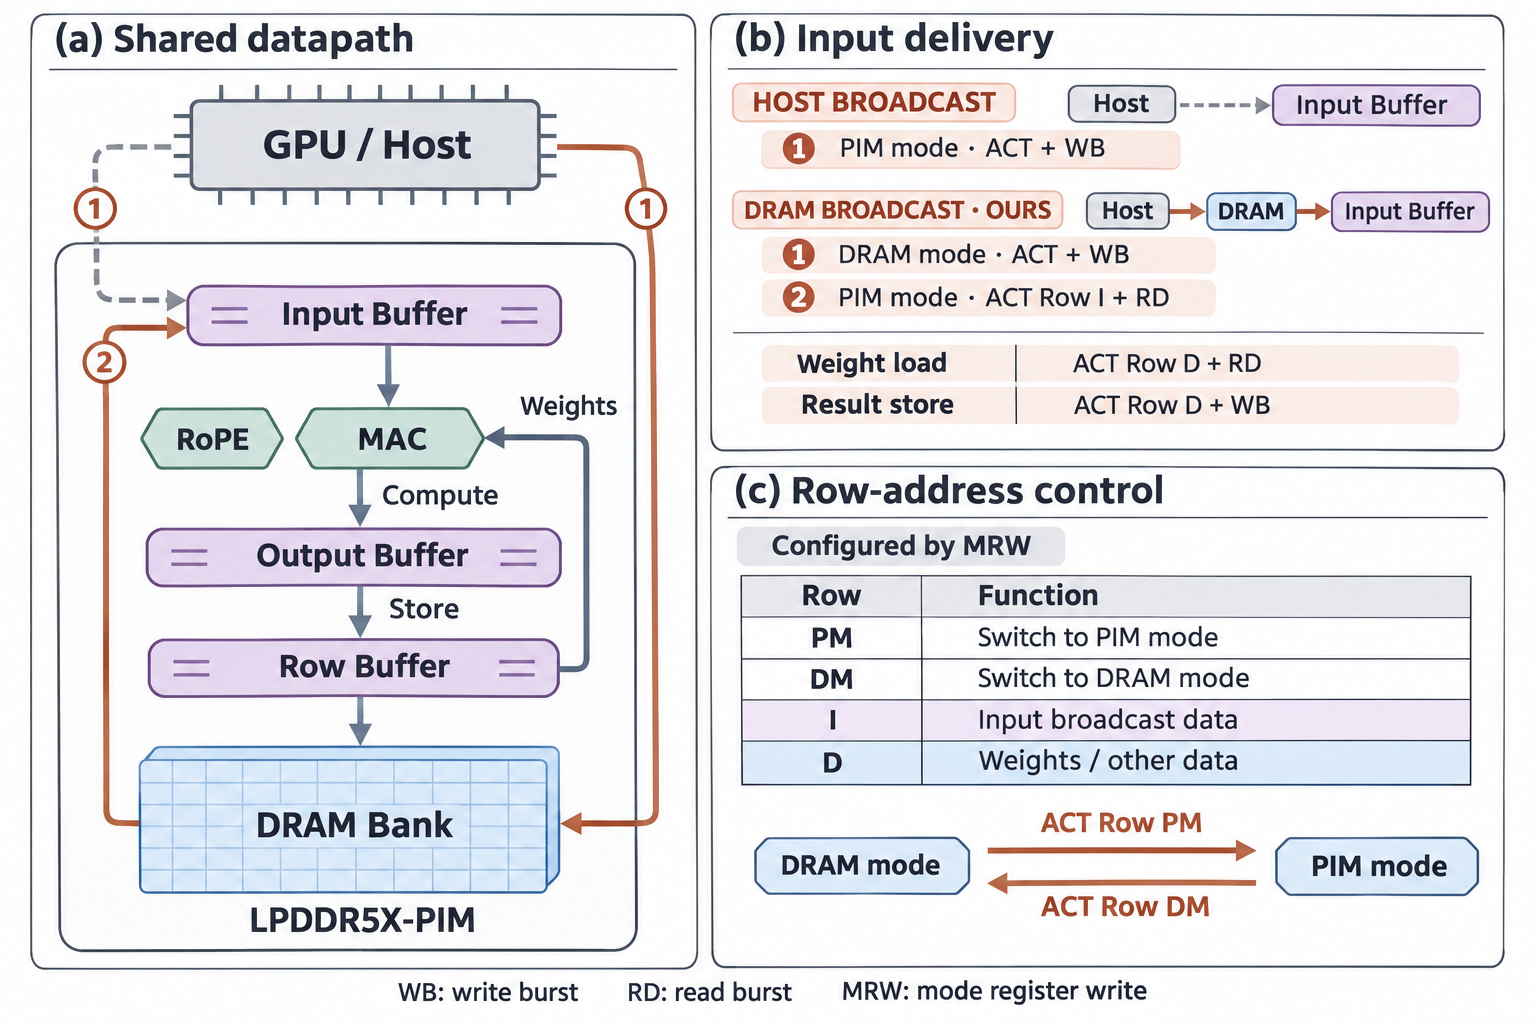
\includegraphics[width=0.82\textwidth]{figures/lpddr5x_pim_B_porcelain.png}
\caption{Input-preloading microarchitecture and function-row control. (a) Shared datapath; (b) host broadcast and in-DRAM broadcast; (c) function rows configured by MRW and mode switching.}
\label{fig:preload}
\end{figure*}

Existing designs such as LPDDR5X-PIM stream inputs from the host, so the DQ bus is intermittently occupied throughout the execution of an operator. This is unfriendly to the frequent rank switching in \sys{}. Either the WCKs of both ranks are kept synchronized at the cost of the power of an idling high-frequency data clock, or every switch pays the time of WCK synchronization and bus read/write (R/W) turnaround. Under JEDEC LPDDR5X-8533 timing, a PIM write followed by a GPU read and then another PIM write incurs a total DQ boundary overhead of 13~CK. Adding one 2-CK read burst, a gap of at least 15~CK is needed to insert a single GPU read. Ramulator simulation shows that, with streaming input, 52.9\% of the gaps between adjacent PIM data bursts are shorter than 15~CK (Fig.~\ref{fig:gap}(a)) and cannot be used to issue any GPU memory request. To exploit the remaining, longer gaps, the memory controller (MC) would additionally need DQ lookahead to predict whether each gap can accommodate the DQ burst of a GPU access, which complicates the arbitration logic.
% REVIEW (Alina Wong, gdoc comment c2 on the v3 draft): the "15 CK" threshold is disputed:
% "it should be at least 5 CK, and by probability the fraction is small". The same claim
% appears in Section V-B and in the Fig. gap caption. Resolve before submission.
\todo{Comment c2: the 15~CK threshold and the 52.9\% figure are disputed.}

\sys{} therefore uses a microarchitecture that suits rank partitioning better. Each bank gets an additional path from the Row Buffer to the Input Buffer, which supports an \emph{input-preloaded} dataflow (Fig.~\ref{fig:preload}):
\begin{enumerate}
\item \textbf{Bulk loading.} While the PIM rank is in DRAM mode, the host writes all inputs of an operator into the input region of the PIM rank (Row~I) at once and at full bandwidth, using ordinary WR commands.
\item \textbf{Local broadcast.} After the PIM rank switches to PIM mode, the MC issues an ACT to Row~I; the column data subsequently read out by RD are broadcast to the Input Buffers of all 16 banks.
\item \textbf{Local compute and write-back.} MAC results are written back to the result region in DRAM. After the computation, the host reads out all results at once in DRAM mode.
\end{enumerate}

This has two benefits. (a)~\textbf{DQ gap fusion.} Input transfers that were scattered across an operator are concentrated at its start. During PIM computation, the DQ bus is returned entirely to the GPU, which obtains long, contiguous access windows. (b)~\textbf{No fine-grained arbitration.} Since the inputs are ready in advance, the MC no longer needs DQ lookahead to decide whether a GPU command fits into a gap.

\textbf{C/A occupancy.} The linear operators of the AE are skinny GEMMs: a single RD column command completes the MAC for all $M$ input rows, so the command density is low. In simulation, the PIM rank occupies only 14.4\% of the external C/A cycles during PIM phases, and 54.4\% together with the C/A traffic of the GPU, so the C/A bus is not saturated. Preloading does not increase the C/A load either: with streaming input, the C/A occupancy of the PIM rank is 16.2\% (Section~\ref{sec:evaluation-b}).
% REVIEW (Alina Wong, gdoc comment c1 on the v3 draft): "This is odd, not what I meant to say.
% I recall running a simulation that replays the trace accounting for C/A occupancy, allowing
% 1-CK delays, etc." Rewrite this paragraph around that replay experiment.
\todo{Comment c1: rewrite this paragraph around the C/A-aware replay simulation.}

\subsection{PIM Command Interface and ISA Extension}
\label{sec:architecture-c}

\sys{} extends the JEDEC LPDDR5X command set with a PIM mode and defines the memory-side command-decoding state machine and ISA.

During LPDDR initialization, the host configures the function rows, including the mode-switch row and the input-buffer row, through Mode Register Writes (MRW). Afterwards, the MC only needs to activate the designated function row to switch a rank between DRAM mode and PIM mode.

In PIM mode, the same RD/WR is executed by all 16 banks in parallel, so the four address bits that normally select the bank group and the bank are unused. \sys{} uses these four bits to encode the operation type (Table~\ref{tab:isa}) and to specify which module writes its result back to DRAM \todo{microarchitecture figure}. All commands keep the JEDEC timing and pin semantics and are therefore compatible with a standard MC.

% Writing note from v3: the opcode table may be turned into a figure in the final version.
% Figure to be drawn: RD command format, marking the four reused BG/BA bits and the column-address bits.
% Local proposal v3; opcode assignments are unchanged.
\begin{table}[!t]
\caption{BG/BA Opcodes of RD/WR in PIM Mode}
\label{tab:isa}
\centering
\footnotesize
\setlength{\tabcolsep}{2.5pt}
\renewcommand{\arraystretch}{0.82}
\setlength{\aboverulesep}{1pt}
\setlength{\belowrulesep}{1pt}
\begin{tabularx}{\columnwidth}{@{}ccl>{\raggedright\arraybackslash}X@{}}
\toprule
\textbf{BG/BA} & \textbf{Cmd.} & \textbf{Operation} & \textbf{Function} \\
\midrule
0000 & RD & \texttt{MAC} & Accumulate MAC result \\
0001 & RD & \texttt{MAC\_INIT} & Initialize accumulator \\
0010 & RD & \texttt{MAC\_RED} & Multi-MAC reduction (reserved) \\
0011 & RD & \texttt{MAC\_INIT\_RED} & Single-MAC dot product + reduction \\
0100 & RD & \texttt{MAC\_INIT\_RED} & Dot/reduce; K BF16 lanes 0--7 \\
0101 & RD & \texttt{MAC\_INIT\_RED} & Dot/reduce; K BF16 lanes 8--15 \\
0110 & RD & \texttt{RD\_ROPE} & Load sin/cos into RoPE registers \\
0111 & RD & \texttt{RD\_ROPE\_Q} & Load and rotate Q \\
1000 & RD & \texttt{RD\_ROPE\_K} & Load and rotate K \\
\midrule
0000 & WR & \texttt{WB\_ACC} & Store accumulator to DRAM \\
0001 & WR & \texttt{WB\_MAC} & MAC bypass to DRAM (reserved) \\
0011 & WR & \texttt{WB\_OBUF} & Store output buffer to DRAM \\
\bottomrule
\end{tabularx}
\par\smallskip
\parbox{\columnwidth}{\scriptsize\mbox{\textit{RD Command:} \texttt{RD16}\,|\,\texttt{BG[1:0]}\,|\,\texttt{BA[1:0]}\,|\,Column Address \texttt{C[5:0]}\,|\,\texttt{AP}}}
\end{table}


\section{Dataflow and Scheduling}
\label{sec:dataflow}
\subsection{DQ-Aware Dataflow: Data Layout and In-Bank RoPE}
\label{sec:dataflow-a}
Because the GPU and PIM share each channel's interface, the AE's data layout also determines DQ contention with the GPU. \sys{} therefore minimizes the AE's external DQ demand under compute and capacity constraints.

Attention tensors can be partitioned across ranks feature-wise, where each rank stores all tokens but half of the feature dimensions, or token-wise, where each rank stores half of the tokens with all feature dimensions. Communication cost in LPDDR-PIM is hierarchical. Intra-rank communication bypasses the DQ bus: inputs are written to all banks at once through the broadcast datapath, and partial sums are reduced by the on-chip adder tree. Inter-rank communication, in contrast, consumes external DQ bandwidth, because without a logic die, cross-rank duplication and reduction must be routed through the MC.

An efficient layout should therefore keep the reduction dimension within a rank and partition only independent dimensions across ranks (\textbf{Fig.~\ref{fig:layout-dq}(a)}). Based on the resulting external DQ traffic, \sys{} adopts the token-wise layout. For attention, it lowers the external DQ traffic per layer and denoising step from $1552\,\mathrm{KiB}$ to $936\,\mathrm{KiB}$, a $39.7\%$ reduction (\textbf{Fig.~\ref{fig:layout-dq}(b)}).

The prefix and suffix KV in the AE also have different lifetimes. The prefix KV is generated once by the VLM and stays read-only across all 10 denoising steps, so its RoPE is applied in the VLM forward pass at no denoising cost. The suffix KV is recomputed from $x_t$ in every layer and step, so its RoPE recurs across 10 steps and 18 layers; running it on the GPU would move Q/K back and forth over the DQ bus. Since RoPE's sine and cosine depend only on the position ID, \sys{} precomputes them into static BF16 lookup tables in the DRAM arrays. Because RoPE needs only MACs between adjacent element pairs, a pair-major feature mapping keeps each pair in one bank for in-place rotation. In-bank RoPE removes another $128\,\mathrm{KiB}$ per layer and step ($2.1\%$), cutting the AE's total DQ traffic from $6096\,\mathrm{KiB}$ to $5224\,\mathrm{KiB}$, a $14.3\%$ reduction.

\subsection{GPU--PIM Co-Scheduling}
\label{sec:dataflow-b}
Building on the input-preloading microarchitecture and the DQ-aware dataflow, \sys{} enables parallel execution through GPU--PIM co-scheduling. Rather than arbitrating individual memory requests, it assigns DQ bus ownership to the GPU or the PIM at kernel granularity. This coarse-grained allocation avoids the complex arbitration, frequent rank switching, and bus turnaround latency caused by interleaving host and PIM commands. \textbf{Fig.~\ref{fig:timeline}} shows the execution sequence within one denoising step.

For $\pi_{0.5}$ with WCK resynchronized at every rank switch, combining all the above techniques reduces the total number of cross-rank switches from $11.845$ million to $28.8$ thousand ($411\times$ fewer) and increases the fraction of the DQ bus occupied by the GPU during PIM computation by $34\%$. Together, these effects improve both speedup and energy efficiency.
% Source: methodology-zh-v3.md, section V
% Chinese text retained; Drive comment metadata is kept only in the local backup.
\section{评估}\label{sec:evaluation}

\subsection{实验设置}\label{sec:evaluation-a}

我们采用``Thor 实测校准 VLM 访存模型 + Ramulator2 周期精确仿真 PIM''的评估方法。GPU 侧，在 NVIDIA Thor 上用 OpenPI 的 PyTorch 实现实测 \(\pi_{0.5}\)（MHA8 配置，BF16，batch=1，动作块长度 H=16，10 个去噪步，3 路相机加 200 个文本 token），得到 VLM 各 kernel 的时长与读写字节，以及 AE 非线性算子的时长。PIM 侧，基于 Ramulator2 构建周期精确仿真器，在同一个内存控制器中同时模拟 VLM 访存与 PIM 命令；DRAM 时序取自 JEDEC JESD209-5C 的 LPDDR5X-8533 速档{[}待引用{]}。

面积评估方面，VLA-PIM相比LPDDR5X，每个 PIM bank 新增 1 KiB Input Buffer、2 KiB Output Buffer、MAC 单元与 RoPE 单元，以及 Row Buffer \(\rightarrow\) Input Buffer 的广播通路。我们沿用 AttAcc 的方法估计面积：先在逻辑工艺下综合新增单元，再按 DRAM 工艺相对逻辑工艺的面积代价折算到 DRAM 裸片上【待核：AttAcc 原文采用的工艺节点、折算系数及其引用来源】。【待补-M11：面积数值】

% Source caption: 表 VII：主要仿真参数
\begin{table}[t]
\centering
\caption{主要仿真参数}
\label{tab:sim-params}
\small
\begin{tabularx}{\linewidth}{@{}>{\raggedright\arraybackslash}p{0.26\linewidth} >{\raggedright\arraybackslash}X@{}}
\toprule
参数 & 取值 \\
\midrule
内存 & LPDDR5X-8533，16 通道 \(\times\) x16，每通道 2 rank，BG 模式 4 BG \(\times\) 4 bank \\
时钟 & CK = 0.938 ns，WCK:CK = 4:1，WCK always-on \\
主要时序 (CK) & CL/CWL 23/12；tRCD 20(读)/9(写)；tRP 20(pb)/23(ab)；tRAS/tRC 45/65；tRRD/tFAW 4/16；tWTR\_\allowbreak{}S/L 7/13；tWR 37；tCCD\_\allowbreak{}L 4 \\
刷新 (CK) & tRFCab/pb 224/128；tREFI/tREFIpb 4164/520 \\
\bottomrule
\end{tabularx}
\end{table}


\subsection{总体性能}\label{sec:evaluation-b}

VLA-PIM 的目标是提高 AE 的推理频率。若每次 AE 推理都使用最新的 VLM KV cache，第 n 帧的 AE 就必须等待第 n 帧的 VLM 完成，因此相邻两次 AE 的间隔为

\begin{equation}
t_{\mathrm{AE\text{-}AE}} = t_{\mathrm{AE,solo}} + t_{\mathrm{VLM,solo}} - t_{\mathrm{overlap}}.
\label{eq:ae-interval}
\end{equation}

其中 \(t_{\mathrm{overlap}}\) 是 VLM 与（上一帧）AE 真正重叠执行的时间。串行执行时 \(t_{\mathrm{overlap}}\) = 0；\(t_{\mathrm{overlap}}\) 越大，AE 的推理频率 1/\(t_{\mathrm{AE\text{-}AE}}\) 越高。表~\ref{tab:performance} 给出各配置的结果。仿真配置的 \(t_{\mathrm{AE,solo}}\) 与 \(t_{\mathrm{VLM,solo}}\) 均取同一设计单独运行的仿真结果（\(t_{\mathrm{VLM,solo}}\) = 65.94 ms）。

% Existing data retained; English captions and references synchronized with the 2026-11-17 source.
\begin{table*}[!t]
\caption{Asynchronous VLA Inference Cycle and AE Output Rate}
\label{tab:performance}
\centering
\footnotesize
\setlength{\tabcolsep}{2.6pt}
\begin{tabular*}{\textwidth}{@{\extracolsep{\fill}}lrrrrrr@{}}
\toprule
\textbf{Config} & \hcell{\textbf{AE done}\\(ms)} & \hcell{\textbf{VLM prog.}\\(ms)} & \hcell{$\bm{t_{\mathrm{overlap}}}$\\(ms)} & \hcell{$\bm{T_{\mathrm{async\_VLA}}}$\\(ms)} & \hcell{\textbf{Rate}\\(Hz)} & \hcell{\textbf{vs.}\\\textbf{a-serial}} \\
\midrule
a-serial (Thor) & 73.98 & --- & 0 & 141.29 & 7.08 & 1.00$\times$ \\
a-dual (Thor) & --- & --- & 4.31 & 137.07 & 7.30 & 1.03$\times$ \\
b & 56.95 & 0 & 0 & 122.88 & 8.14 & 1.15$\times$ \\
c & 60.33 & 47.48 & 36.12 & 86.77 & 11.53 & 1.63$\times$ \\
d & 57.90 & 47.42 & 36.33 & 84.04 & 11.90 & 1.68$\times$ \\
e & 56.83 & 47.16 & 36.35 & 83.57 & 11.97 & 1.69$\times$ \\
f & 69.27 & 60.15 & 54.80 & 78.17 & 12.79 & 1.81$\times$ \\
\textbf{g (\sys{})} & 68.64 & 60.30 & 54.96 & \textbf{77.68} & \textbf{12.87} & \textbf{1.82}$\bm{\times}$ \\
\bottomrule
\end{tabular*}
\par\smallskip
\parbox{\textwidth}{\scriptsize ``VLM prog.'' is the VLM progress completed before the AE finishes.}
\end{table*}


主要观察如下：

\begin{enumerate}
\def\labelenumi{\arabic{enumi}.}

\item
  \textbf{异构本身的收益。} 把 AE 的线性层搬到 PIM 后，即使串行执行（b），\(t_{\mathrm{AE\text{-}AE}}\) 也比 a-serial 缩短到 1/1.15：AE 完成时间为 56.95 ms，而 Thor 上 compile 后的 AE 实测为 73.98 ms；其中 PIM 部分 46.01 ms，占 AE 时间的 80.8\%。
\item
  \textbf{rank 划分带来的并发收益。} 让 VLM 与 AE 并发（c），\(t_{\mathrm{overlap}}\) 达到 36.12 ms，\(t_{\mathrm{AE\text{-}AE}}\) 从 122.88 ms 降到 86.77 ms（1.42\(\times\)）。AE 本身只慢了 3.38 ms（5.9\%），其中 PIM 阶段因 GPU 并发只被拉长 0.51 ms，说明 rank 划分确实为两者提供了相对独立的资源。
\item
  \textbf{布局与 RoPE。} 在流式数据流下，token-wise 布局（d）比 feature-wise（c）快 2.73 ms（3.1\%），片内 RoPE（e）再快 0.47 ms。收益主要来自 AE 侧：DQ 流量减少，GPU 非线性工作从 10.93 ms 降到 8.11 ms。
\item
  \textbf{输入预装载。} 预装载（g）让 AE 的 PIM 部分变长，AE 完成时间增加 11.8 ms；但 AE 结束时 VLM 已完成 60.30 ms 的工作（流式只有 47.16 ms，+27.8\%），\(t_{\mathrm{overlap}}\) 从 36.35 ms 增加到 54.96 ms（+51.2\%）；1416 个 VLM kernel 中完成了 1366 个（流式为 1271 个），剩余的 VLM 尾部从 26.74 ms 缩短到 9.03 ms。最终 \(t_{\mathrm{AE\text{-}AE}}\) 从 83.57 ms 降到 77.68 ms（-7.0\%），AE 推理频率达到 a-serial 的 1.82\(\times\)、a-dual 的 1.76\(\times\)。
\end{enumerate}

\begin{figure*}[!t]
\centering
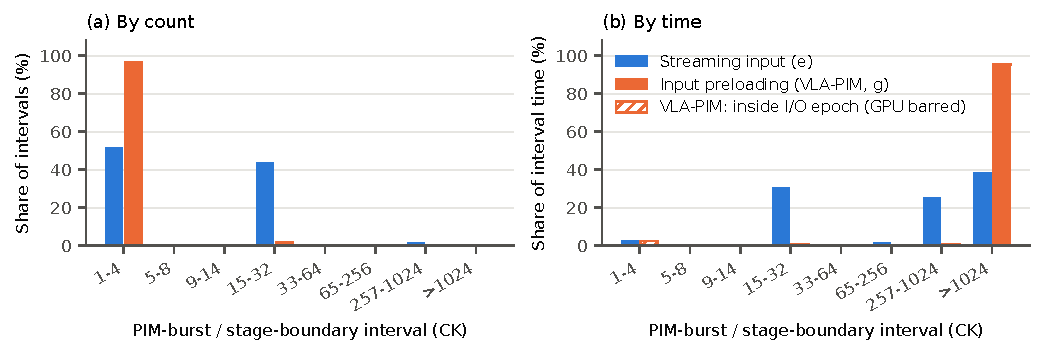
\includegraphics[width=\textwidth]{figures/fig_dq_gap_distribution.pdf}
\setcounter{figure}{7}
\caption{PIM 相邻数据突发间隔的分布（物理通道 0，完整 18 \(\times\) 10 调度）。(a) 按数量；(b) 按时间，斜线部分为位于 I/O epoch 内的间隔。虚线左侧（\textless{} 15 CK）的间隔无法插入一次 GPU 读。}\label{fig:dq-gaps}
\end{figure*}


\textbf{GPU 在 PIM 计算期间获得的带宽。} 我们统计所有 PIM 阶段内（16 通道合计）GPU 获得的 DQ 带宽。VLM 单独运行时，GPU 平均获得 221.6 GB/s。流式供数下，PIM 阶段内 GPU 只能获得 173--175 GB/s，保持率为 78.2\%--78.9\%；预装载后提高到 204.2 GB/s，保持率为 92.2\%。同时，PIM 阶段内 GPU 搬运的数据从 7.53 GiB 增加到 11.35 GiB（+50.7\%）。这说明预装载把原本碎片化、GPU 无法利用的 DQ 空隙合并成了 GPU 可以连续使用的窗口。

\textbf{DQ 空隙分布。} 图~\ref{fig:dq-gaps} 统计了完整 18 层 \(\times\) 10 步调度中，物理通道 0 上 PIM 相邻数据突发之间的间隔。流式供数（e）下共有 126 万个间隔，其中 52.9\% 短于 15 CK，按 DQ 时序无法插入任何一次 GPU 读；按时间计，只有 38.8\% 的间隔时间落在长于 1024 CK 的窗口中。预装载（g）后，间隔数减少到 77 万个（-38.7\%）。虽然按数量计 97.2\% 的间隔短于 15 CK，但它们都是 I/O epoch 内连续传输之间的间隔，而 GPU 在 epoch 内本就不发请求；在 epoch 之外，99.8\% 的间隔时间落在长于 1024 CK 的窗口中。需要说明的是，这些间隔中可能已经包含 GPU 的传输，因此``无法插入 GPU 读''只是基于 DQ 时序的几何判断，并非实测的 GPU 不可用时间。


\textbf{C/A 占用。} 在 PIM 阶段内，PIM rank 占用的外部 C/A 周期比例为：c 14.2\%、d 16.2\%、e 16.2\%、f 14.4\%、g 14.4\%。g 中加上 GPU 的 C/A 占用（40.0\%），C/A 总占用为 54.4\%，C/A 总线仍有余量。预装载在为 GPU 释放 DQ 的同时，并未增加 C/A 负担。

\subsection{讨论：VLM 与 AE 的解耦}\label{sec:evaluation-c}

\begin{figure}[!t]
\centering
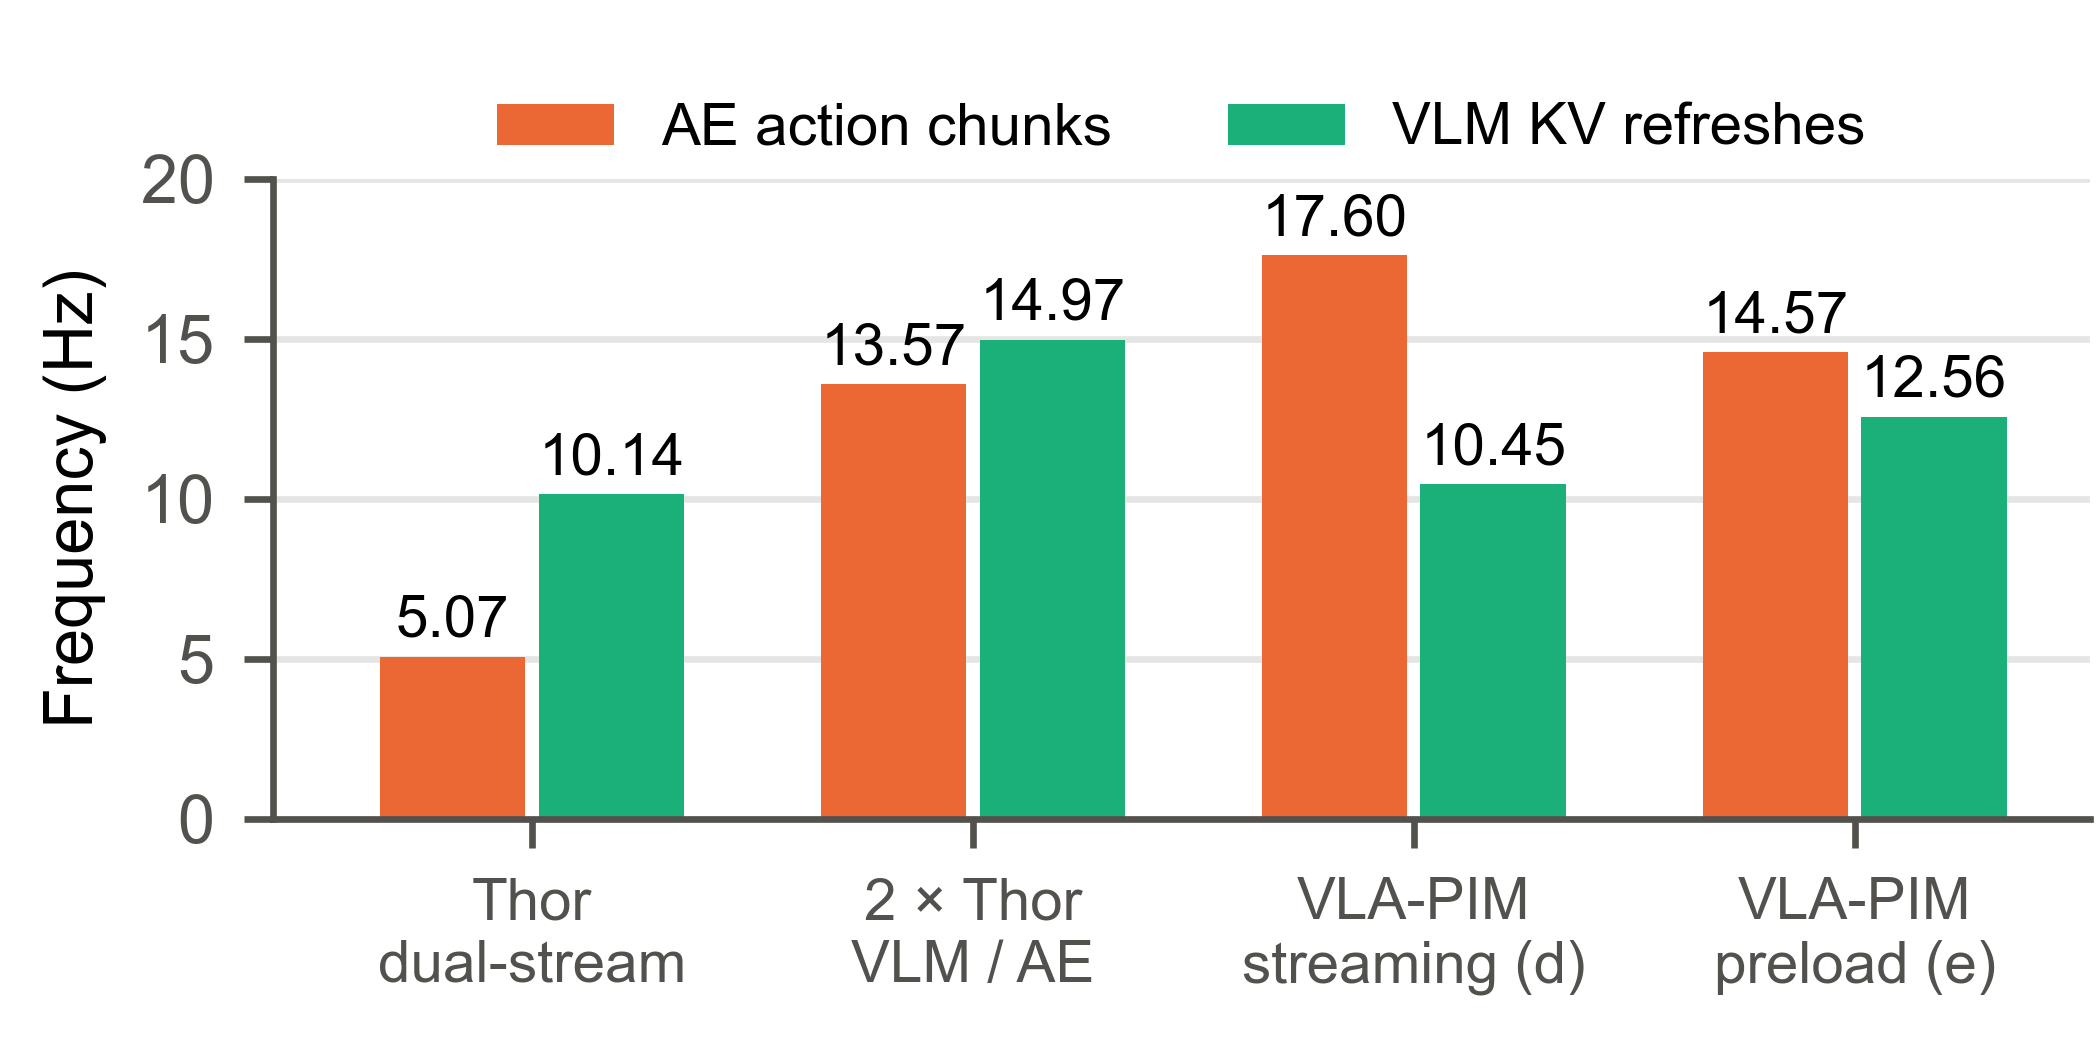
\includegraphics[width=\columnwidth]{figures/fig8_decoupled_rate.png}
\caption{AE action-chunk rate and VLM KV refresh rate under decoupled execution.
Thor dual-stream: VLM and AE sharing one GPU;
2$\times$ Thor: dedicated GPUs for VLM and AE.}
\label{fig:decoupled-rates}
\end{figure}


VLA-PIM 的异构结构天然支持 VLM 与 AE 解耦。配合合适的异步算法，VLM 可以较慢地更新 KV cache，PIM 则以更高的频率执行 AE 推理，实现真正的异步执行。单 GPU 上则很难做到：Thor 双 stream 连续运行时，AE 只有 5.13 Hz，VLM 刷新频率为 10.13 Hz。增加 GPU 算力也无法缓解 AE 的访存受限：即使让 AE 独占 Thor GPU，其频率也只有 13.57 Hz。在 VLA-PIM 中，AE 与 VLM 解耦运行时，AE 频率约为 14.57 Hz，是 Thor 双流的 2.84\(\times\)，并超过 AE 独占 GPU 的频率；同时 VLM 刷新频率约为 12.56 Hz，只比 VLM 独占 GPU（14.97 Hz）低 16.1\%，比 Thor 双流高 24.0\%（图~\ref{fig:decoupled-rates}）。也就是说，VLA-PIM 只让 GPU 上 VLM 的更新频率下降约 1/6，就使 AE 推理频率达到双流 GPU 基线的近 3 倍。这里的频率由单个重叠窗口外推得到：AE 频率取 1/AE 完成时间，VLM 频率按窗口内完成的 VLM 工作量折算，尚未做多帧连续仿真。

% English translation of essay/ActPIM_初稿_v3.md, Section VII.
\section{Conclusion}
\label{sec:conclusion}

This paper presents \sys{}, which jointly organizes the GPU memory accesses of the VLM and the PIM computation of the AE within an edge LPDDR memory system. Rank partitioning keeps all channels available to feed the GPU. The shared-bus-aware token-wise layout and the lifetime-aware in-memory RoPE reduce the per-layer DQ traffic of the AE by 14.3\% (21.7\% together with input preloading). Input preloading and kernel-granularity co-scheduling concentrate the remaining transfers, so the GPU retains 92.2\% of its standalone bandwidth during PIM computation. By combining a lower transfer volume with organized transfer timing, this design broadens the goal of heterogeneous execution: beyond accelerating the AE, it overlaps PIM computation effectively with GPU execution while sustaining the GPU's memory service. Based on Thor measurements and cycle-accurate simulation, \sys{} achieves an AE inference rate of $1.82\times$ that of serial execution on Thor and $1.76\times$ that of the dual-stream GPU baseline.

\StopChinese
\end{document}
